\begin{titlepage}
    \begin{center}
        %\vspace*{0.5cm}
       
        {\LARGE\textbf{Characterisation of a\\}}
        %\vspace{0.1cm}
        {\huge\textbf{Cold-Atom Electron Source\\}}
        %\vspace{0.1cm}
        {\LARGE\textbf{for\\}}
        %\vspace{0.1cm}
        {\huge\textbf{Ultrafast Diffractive Imaging\\}}
    
        \vspace{2cm}
        
        \href{https://scholar.google.com.au/citations?user=sLp309oAAAAJ}{{\huge Joshua Stephen Jones \textsc{Torrance}}}

        \vspace{0.3cm}

        ORCID: \href{http://orcid.org/0000-0002-0463-2967}{0000-0002-0463-2967}
        
        \vfill
        
        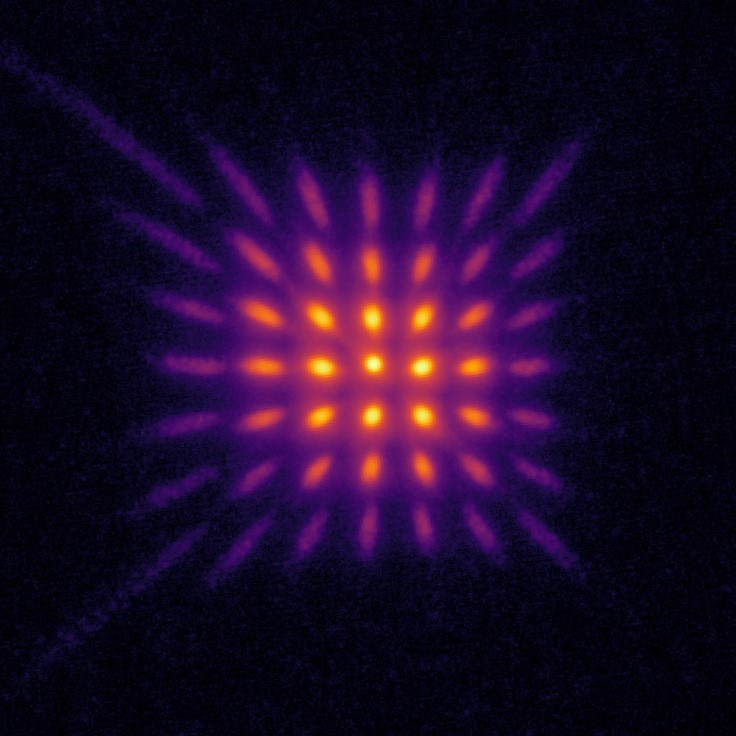
\includegraphics[width=5cm]{0frontmatter/example_pepperpot_detector_linear.jpeg}

        \vfill

        Submitted in total fulfilment of the requirements
        of the degree of Doctor of Philosophy

        \vspace{0.4cm}

        \href{http://physics.unimelb.edu.au}{School of Physics\\
           The University of Melbourne}\\
        
        \vspace{0.4cm}
    
        \today

        \vspace{0.4cm}

        Supervised by \href{https://scholar.google.com.au/citations?user=F3QFcRYAAAAJ}{Professor Robert E. Scholten}
        and \href{https://scholar.google.com.au/citations?user=pqsudawAAAAJ}{Doctor Benjamin M. Sparkes}       
    \end{center}
\end{titlepage}